\documentclass[12pt, a4paper]{article}

\usepackage[
  margin=1in
]{geometry}

\usepackage[T1, T2A]{fontenc}
\usepackage[utf8]{inputenc}
\usepackage[russian]{babel}
\usepackage{minted}
\usepackage{tabularray}
\usepackage{siunitx}
\usepackage{graphicx}
\usepackage{multicol}

\graphicspath{ {img/} }

\begin{document}

\begin{titlepage}
  \centering
  \textsc{Новосибирский государственный технический университет}\par
  \vspace{1mm}
  Кафедра прикладной математики\par
  \vspace{4cm}
  \textsc{Практическая работа \textnumero 6}\par
  {\huge\bfseries Параллельные алгоритмы на графах\par}
  \vspace{1cm}
  {\scriptsize ФПМИ, ПМ-24\par}
  \vspace{1mm}
  {\itshape\large Параскун И., Шакиров П., Герасименко В.\par}
  \vfill
  {\small преподаватель\par}
  \vspace{1mm}
  \textsc{Домников Петр Александрович}
  \vfill
  \large{Новосибирск, 2024}
\end{titlepage}

\newpage
\setcounter{page}{2}

\section{Постановка задачи}
Написать параллельный алгоритм Дейкстры для поиска кратчайших путей между всеми парами вершин графа.
\begin{itemize}
  \item Граф хранится в виде списков смежности;
  \item Результат работы программы - матрица кратчайших путей;
  \item Инструмент параллельных вычислений - OpenMP.
\end{itemize}

\section{Текст программы}

\inputminted[firstline=7, lastline=32]{c}{/home/mehandes/c/src/github.com/meha4j/math/bgs/dcg/include/bgs/dcg.h}
\inputminted[firstline=61, lastline=172]{c}{/home/mehandes/c/src/github.com/meha4j/math/bgs/dcg/src/dcg.c}

\section{Результат работы программы}

\vspace{5mm}
\begin{multicols}{2}
  \begin{flushright}
    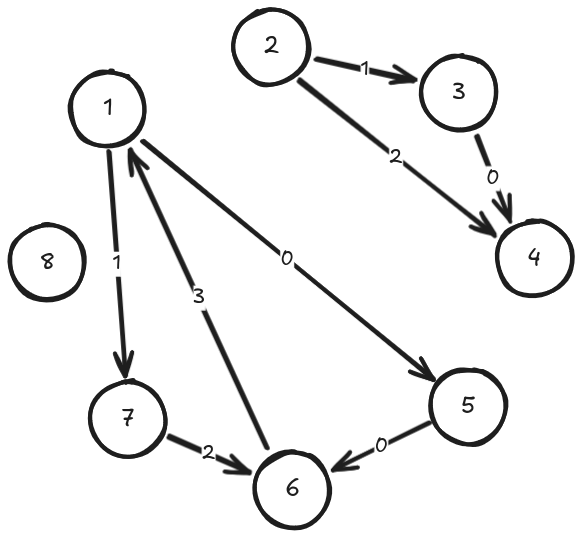
\includegraphics[scale=0.3]{./img/1.png}
  \end{flushright}
\columnbreak
  \begin{flushleft}
    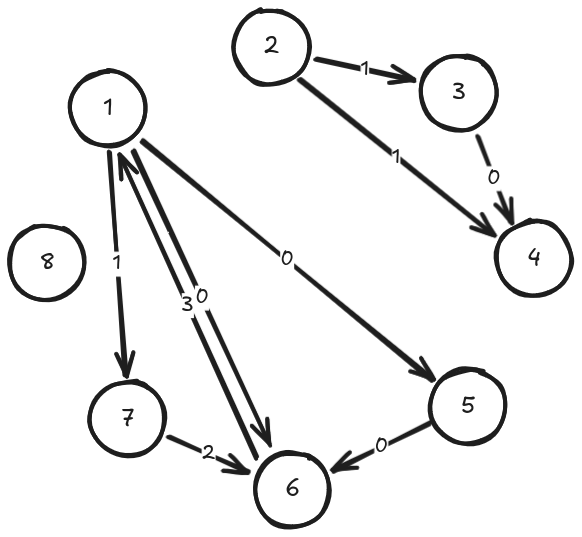
\includegraphics[scale=0.3]{./img/2.png}
  \end{flushleft}
\end{multicols}
\vspace{5mm}

\begin{minted}{console}
1 -> 1 [0]: 1 - 1
1 -> 5 [0]: 1 - 5
1 -> 6 [0]: 1 - 5 - 6
1 -> 7 [1]: 1 - 7
2 -> 2 [0]: 2 - 2
2 -> 3 [1]: 2 - 3
2 -> 4 [1]: 2 - 3 - 4
3 -> 3 [0]: 3 - 3
3 -> 4 [0]: 3 - 4
4 -> 4 [0]: 4 - 4
5 -> 5 [0]: 5 - 5
5 -> 6 [0]: 5 - 6
6 -> 1 [3]: 6 - 1
6 -> 6 [0]: 6 - 6
7 -> 6 [2]: 7 - 6
7 -> 7 [0]: 7 - 7
8 -> 8 [0]: 8 - 8
\end{minted}

\section{Тексты вспомогательных структур данных}

\subsection{Очередь по приоритетам}
\inputminted[firstline=4, lastline=88]{c}{/home/mehandes/c/src/github.com/meha4j/math/gds/include/gds/pque.h}
\inputminted[firstline=6, lastline=150]{c}{/home/mehandes/c/src/github.com/meha4j/math/gds/src/ppque.c}

\subsection{Хеш-множество}
\inputminted[firstline=6, lastline=65]{c}{/home/mehandes/c/src/github.com/meha4j/math/gds/include/gds/hset.h}
\inputminted[firstline=7, lastline=84]{c}{/home/mehandes/c/src/github.com/meha4j/math/gds/src/ihset.c}

\end{document}

